%--------------------
% Packages
% -------------------
\documentclass[12pt,a4paper]{article}
% \usepackage[a4paper, left=15mm, right=15mm, top=15mm, bottom=15mm]{geometry}
\usepackage[utf8x]{inputenc}
\usepackage[T1]{fontenc}
%\usepackage{gentium}
\usepackage{mathptmx} % Use Times Font
% \usepackage[siunitx]{circuitikz} % for circuit schematics
\usepackage{siunitx}
\usepackage{amsmath} % for the equation* environment
\usepackage{graphicx}
\usepackage{pgfplots}
\pgfplotsset{compat=1.14}
\usepackage{float}

\usepackage{graphicx} % Required for including pictures % clashes with circuitikz
% \usepackage[swedish]{babel} % Swedish translations
\usepackage[pdftex,linkcolor=black,pdfborder={0 0 0}]{hyperref} % Format links for pdf
\usepackage{calc} % To reset the counter in the document after title page
\usepackage{enumitem} % Includes lists

\frenchspacing % No double spacing between sentences
\linespread{1.2} % Set linespace
\usepackage[a4paper, lmargin=0.08\paperwidth, rmargin=0.08\paperwidth, tmargin=0.08\paperheight, bmargin=0.08\paperheight]{geometry} %margins
%\usepackage{parskip}
% \usepackage[all]{nowidow} % Tries to remove widows
\usepackage[protrusion=true,expansion=true]{microtype} % Improves typography, load after fontpackage is selected

\usepackage[inkscapelatex=false]{svg}
\graphicspath{ {./media/} }

% \pagecolor{black}
% \color{white}

\usepackage{setspace}


%-----------------------
% Set pdf information and add title, fill in the fields
%-----------------------
\hypersetup{ 	
pdfsubject = {},
pdftitle = {ee5311-2025-ee24s053-pwc-report-tut5},
pdfauthor = {Karthik B K <ee24s053@smail.iitm.ac.in>}
}

%-----------------------
% Begin document
%-----------------------
\begin{document}

\title{EE5311 \\ Report of Practical Work Conducted for Tutorial 05}
\author{Karthik B K ee24s053}
\maketitle

\section{Experiment 01}
\subsection{Stick Diagrams}
\noindent We draw the following stick diagrams for a static CMOS inverter.
\begin{center}
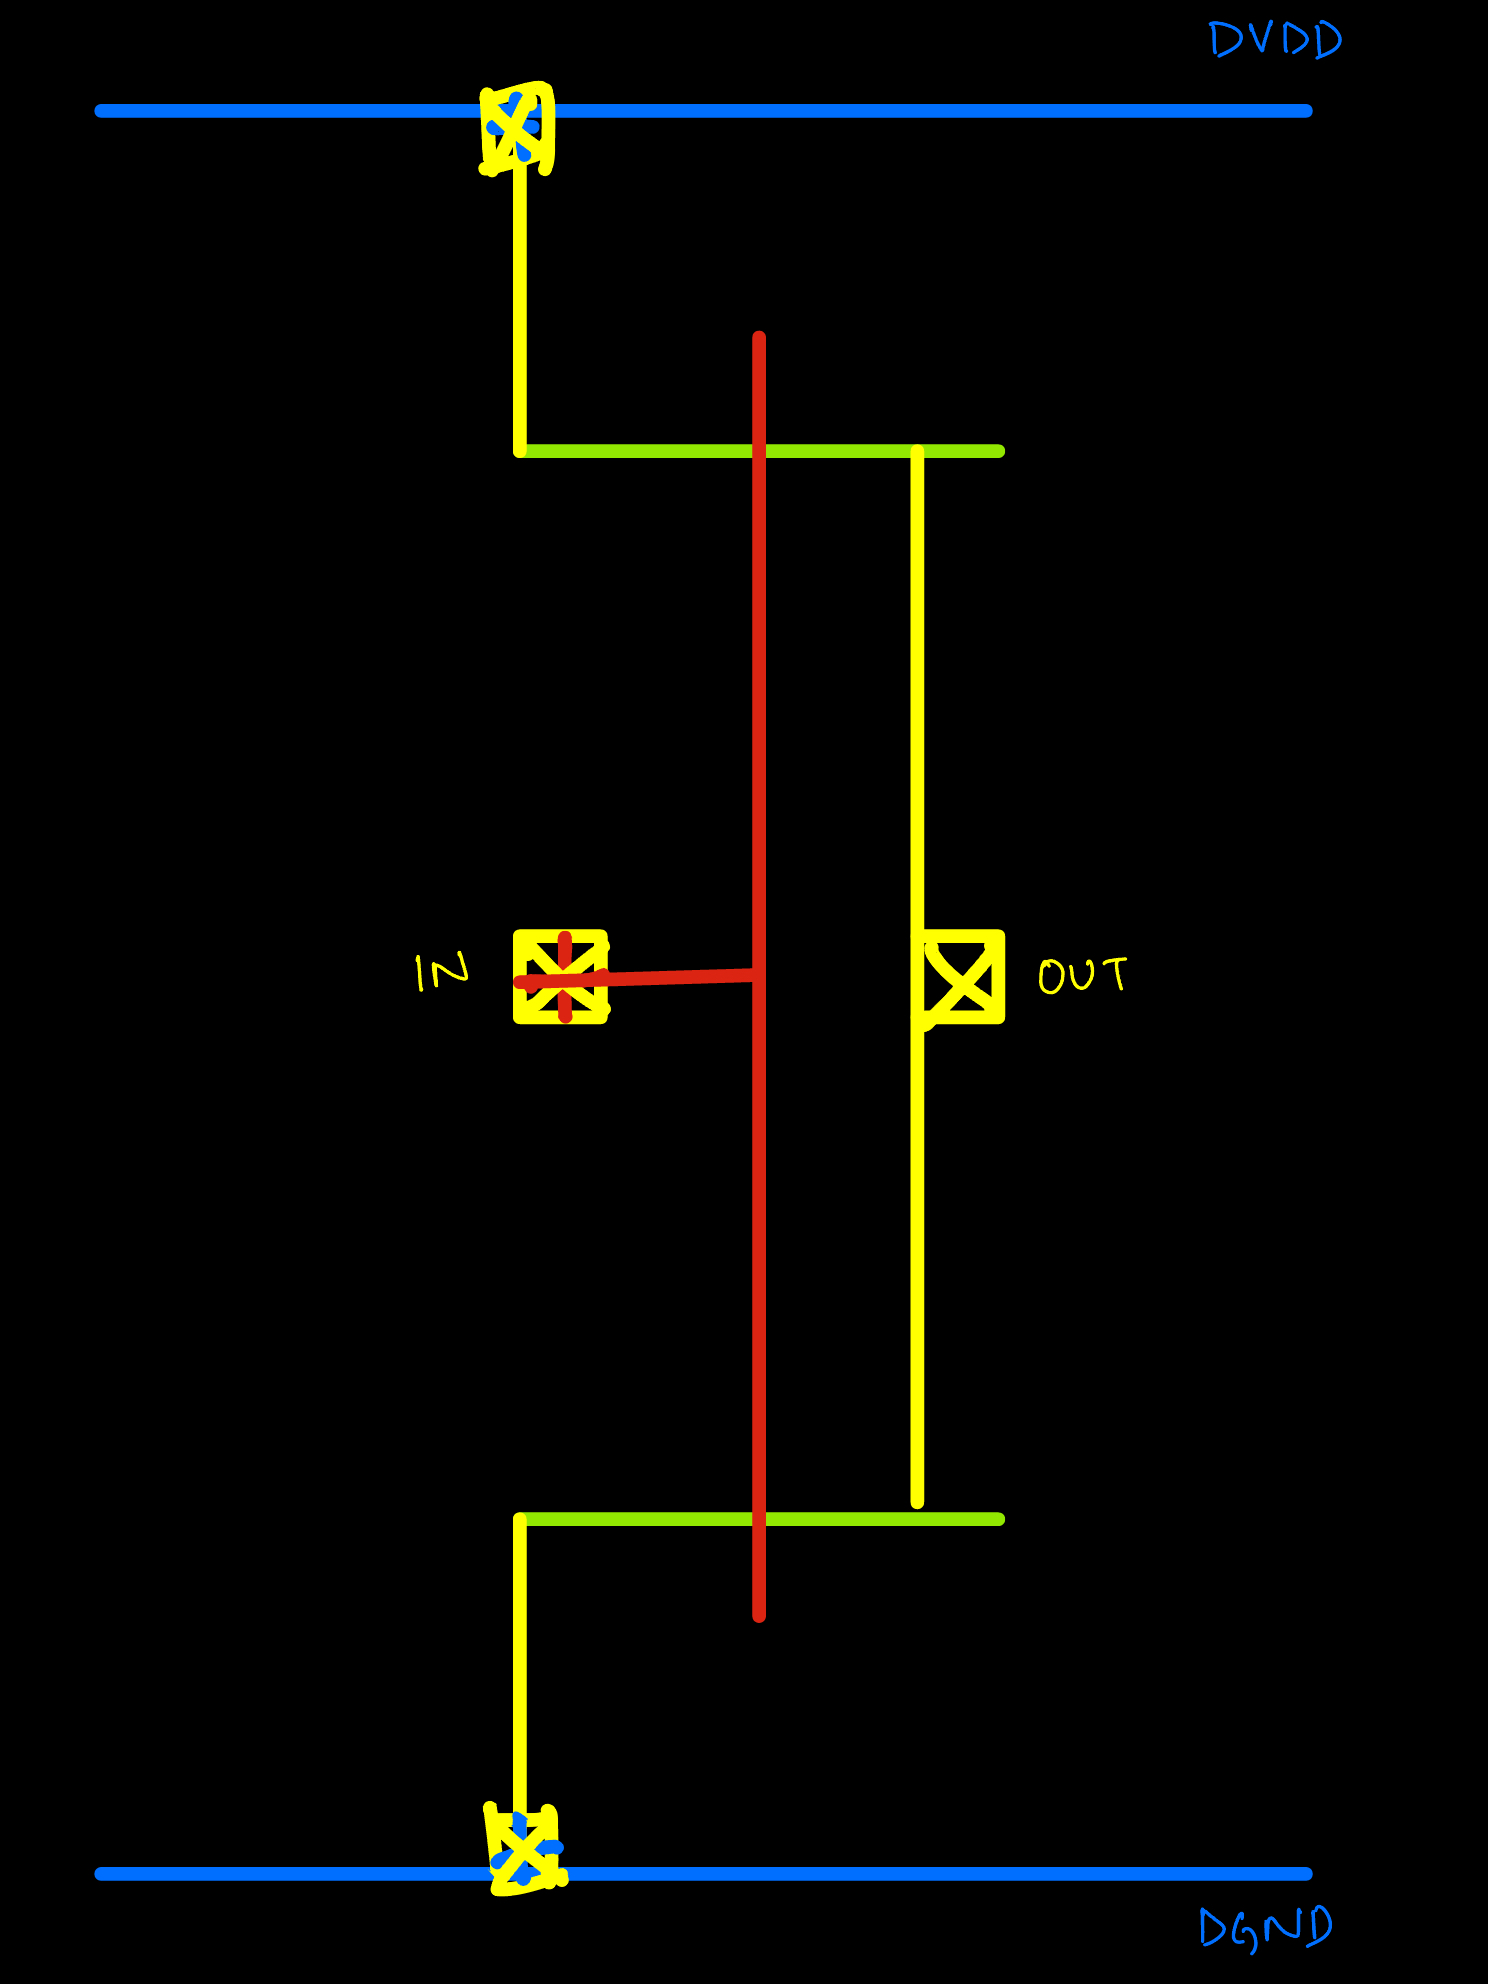
\includegraphics[width=0.29\linewidth]{tut5/reports/media/inv.stick-diagram.jpeg} \\
Fig 1: Layout plan of a static CMOS inverter
\end{center}

\subsection{Layouts}
\noindent We draw the following layout for an inverter using \emph{klayout}.
\begin{center}
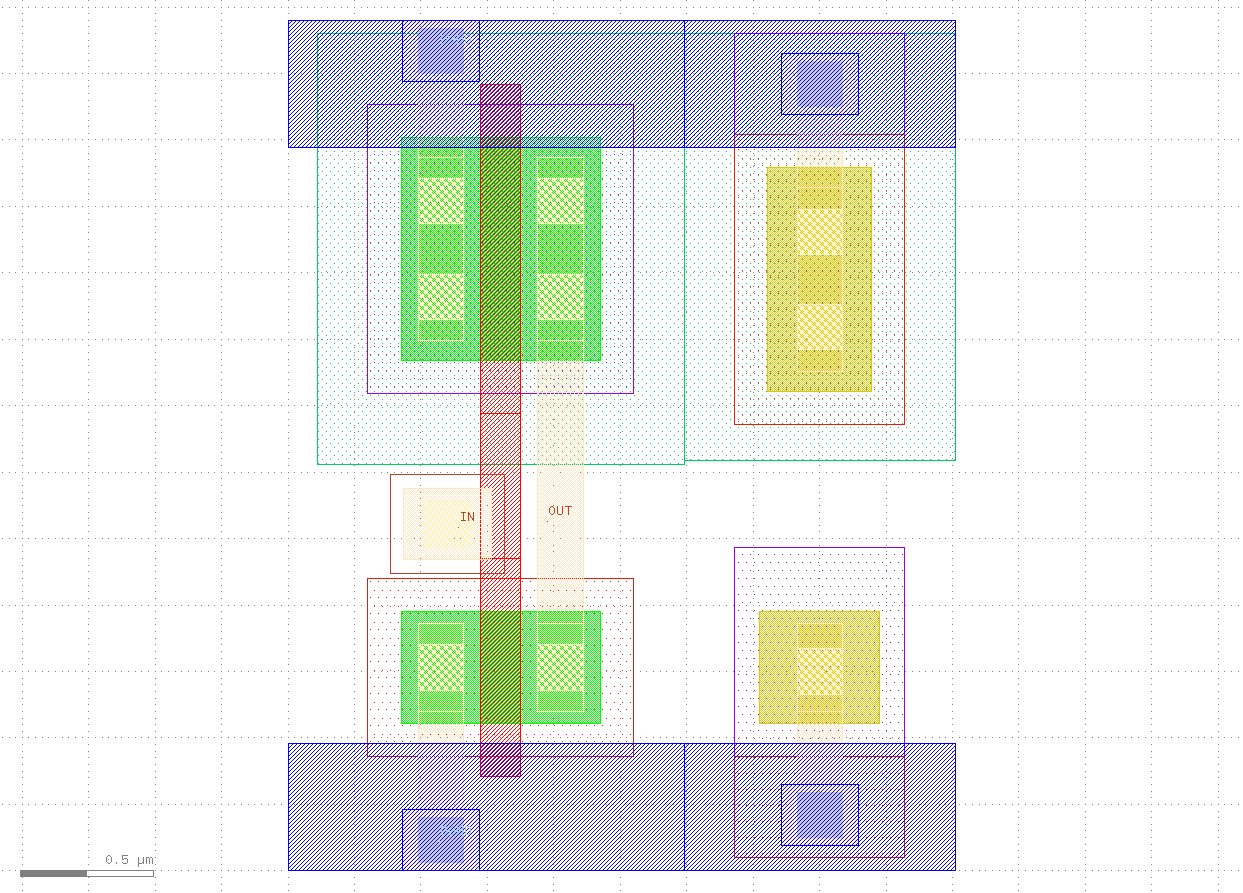
\includegraphics[width=0.49\linewidth]{tut5/inv/cell/subcircuit/inv.gds.png} \\
Fig 2: Layout of a static CMOS inverter
\end{center}

\subsection{Measurements}
\noindent We perform a transient simulation with the setup both before and after layout extraction for the inverter and obtain the following plots.
\begin{center}
\begin{tabular}{cc}
     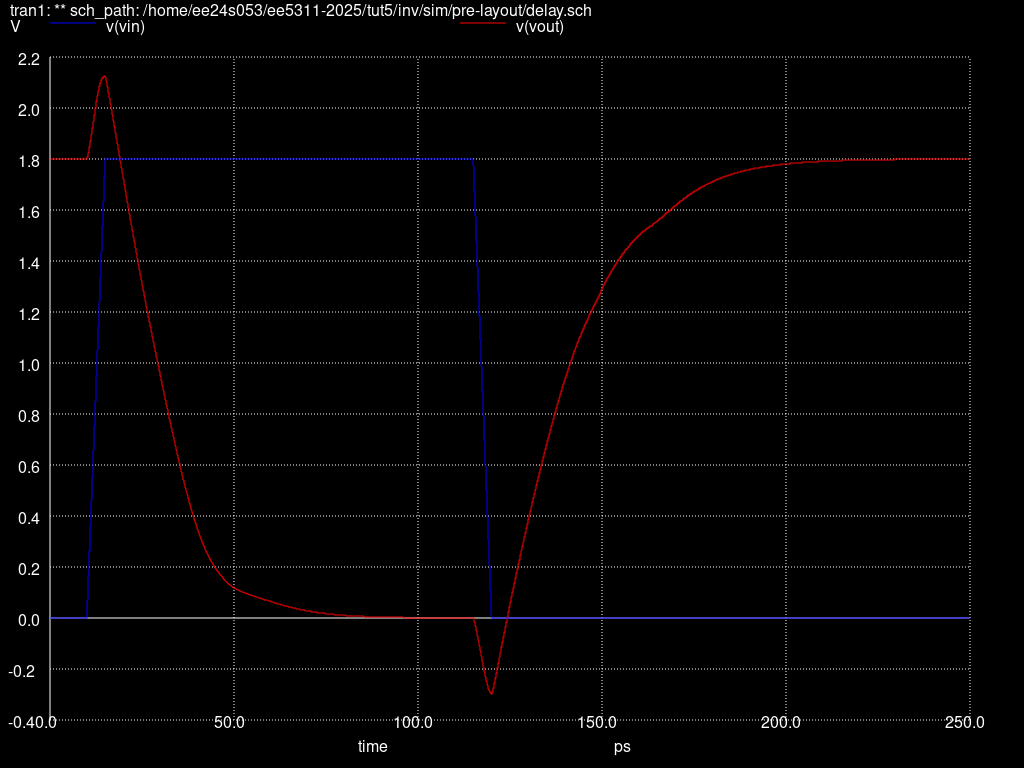
\includegraphics[width=0.47\linewidth]{tut5/reports/media/inv.pre-layout.png} &
     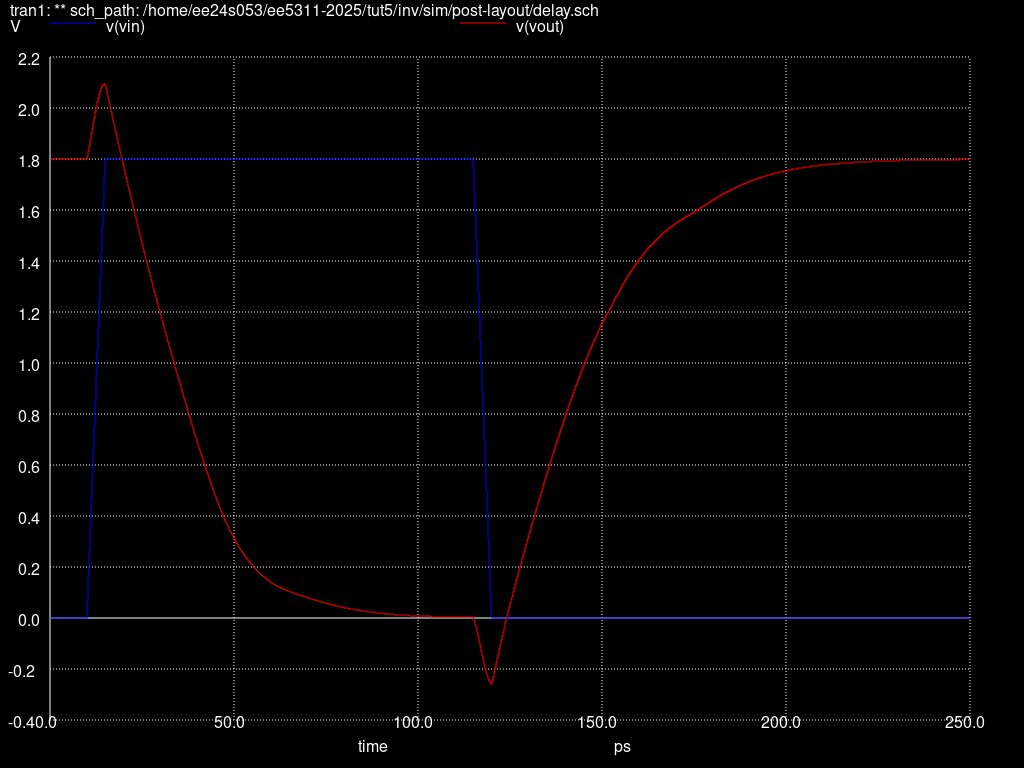
\includegraphics[width=0.47\linewidth]{tut5/reports/media/inv.post-layout.png} \\
     Fig 3a: Transient of an inverter pre-layout & Fig 3b: Transient of an inverter post-layout
\end{tabular}
\end{center}
\noindent We obtain the following values for period and frequency without the layout parasitics.
\begin{verbatim}
    When Vdd = 1.8 V,
        delay = 19.95 ps
        freq = 1/period = 50.12 GHz
\end{verbatim}
\noindent We obtain the following values for period and frequency when we include the layout parasitics.
\begin{verbatim}
    When Vdd = 1.8 V,
        delay = 24.19 ps
        freq = 1/period = 41.33 GHz
\end{verbatim}

\section{Experiment 02}
\subsection{Stick Diagrams}
\noindent We draw the following stick diagrams for a seven stage ring-oscillator. Most of the layout plan is simply a replica of the inverter's layout plan, and the nets highlighted in the plan are the ones that really need an additional connection.
\begin{center}
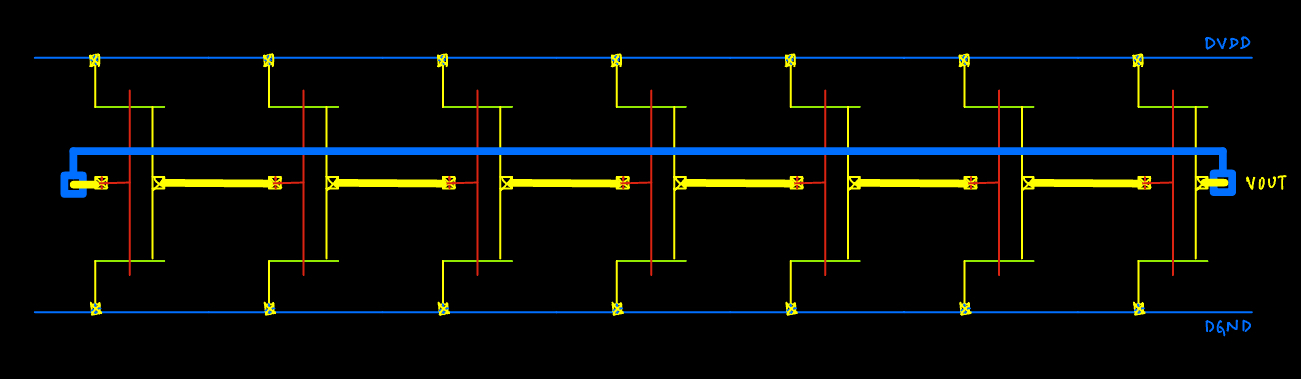
\includegraphics[width=0.99\linewidth]{tut5/reports/media/ro7.stick-diagram.jpg} \\
Fig 4: Layout plan of a seven-stage ring oscillator
\end{center}

\subsection{Layouts}
\noindent We draw the following layout for an inverter using \emph{klayout}.
\begin{center}
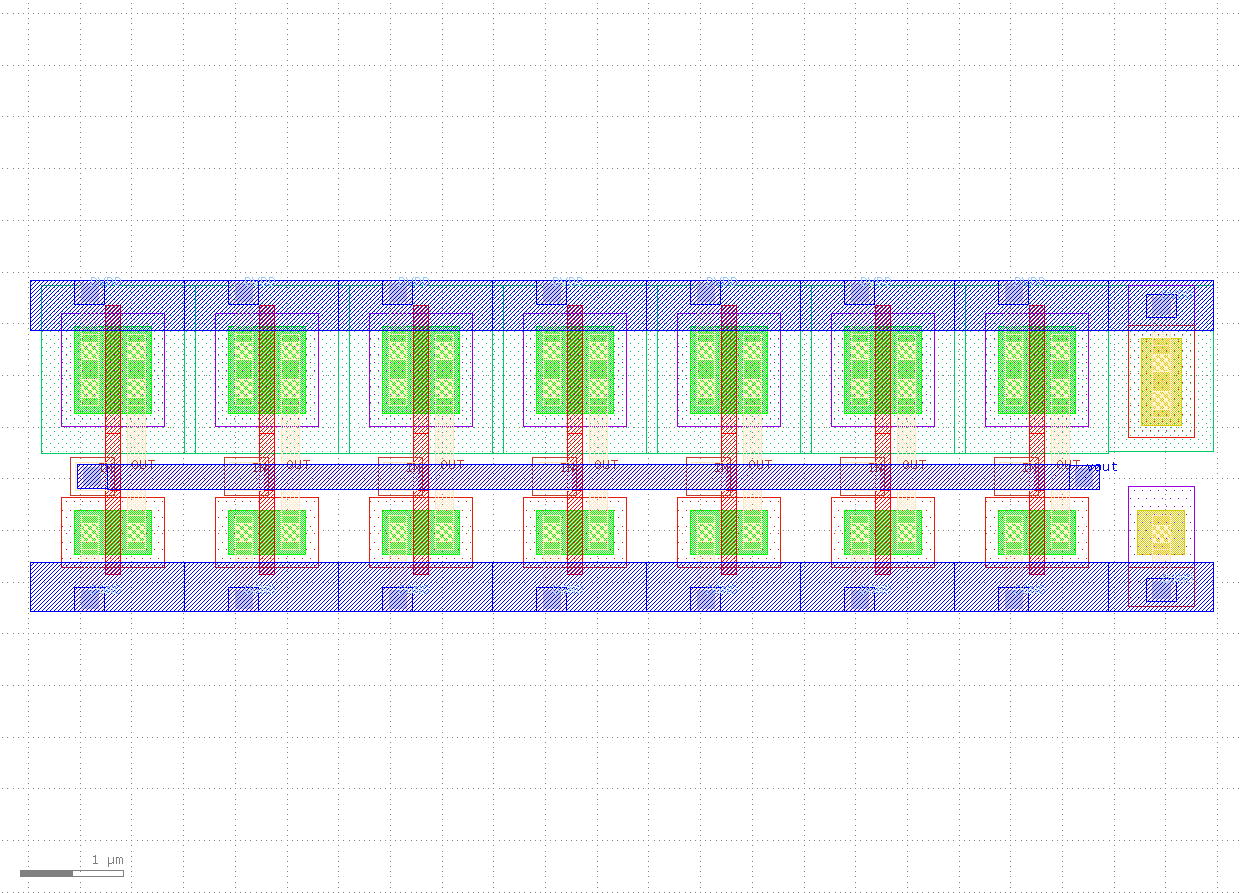
\includegraphics[width=0.99\linewidth]{tut5/ro7/cell/ro7.gds.png} \\
Fig 5: Layout of a Seven-Stage Ring Oscillator
\end{center}

\subsection{Measurements}
\noindent We perform a transient simulation with the setup both before and after layout extraction for the seven-stage ring-oscillator and obtain the following plots.
\begin{center}
\begin{tabular}{cc}
     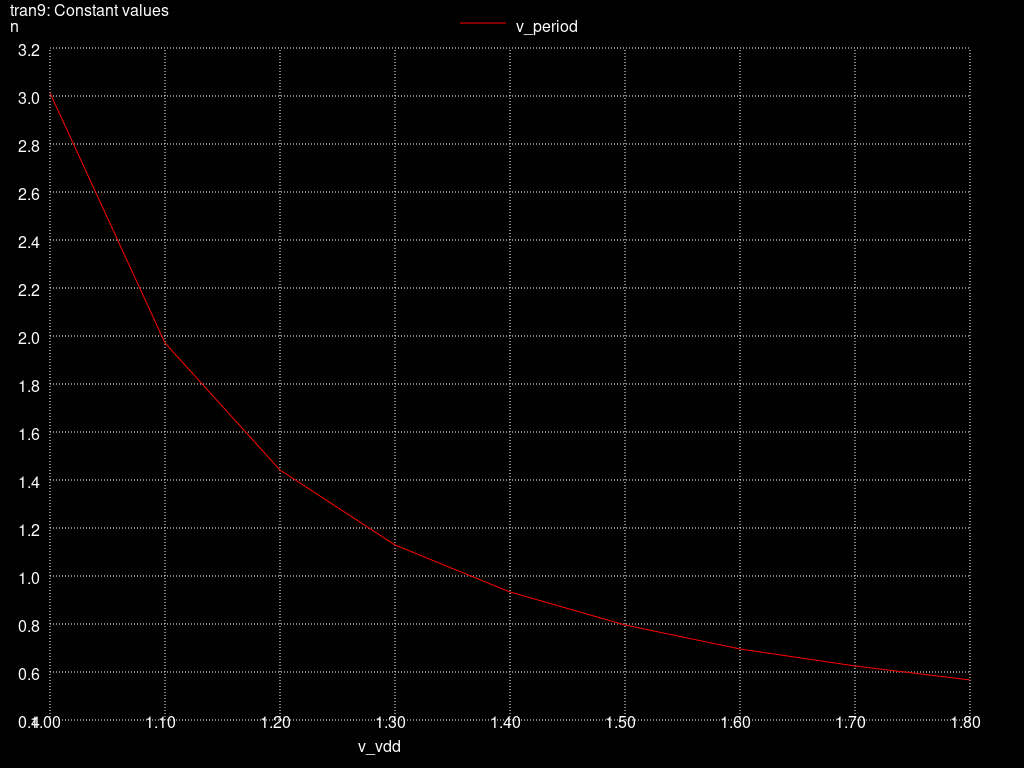
\includegraphics[width=0.47\linewidth]{tut5/reports/media/ro7.pre-layout.period.png} &
     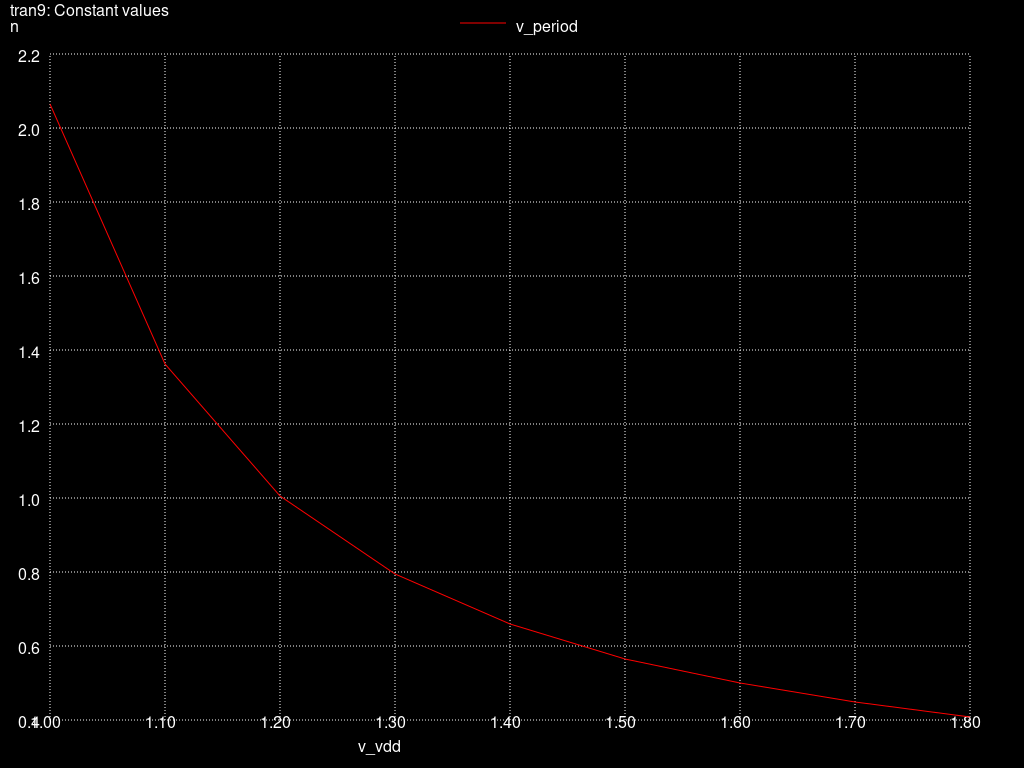
\includegraphics[width=0.47\linewidth]{tut5/reports/media/ro7.post-layout.period.png} \\
     Fig 6a: Period of the circuit pre-layout & Fig 6b: Period of the circuit post-layout
\end{tabular}
\begin{tabular}{cc}
     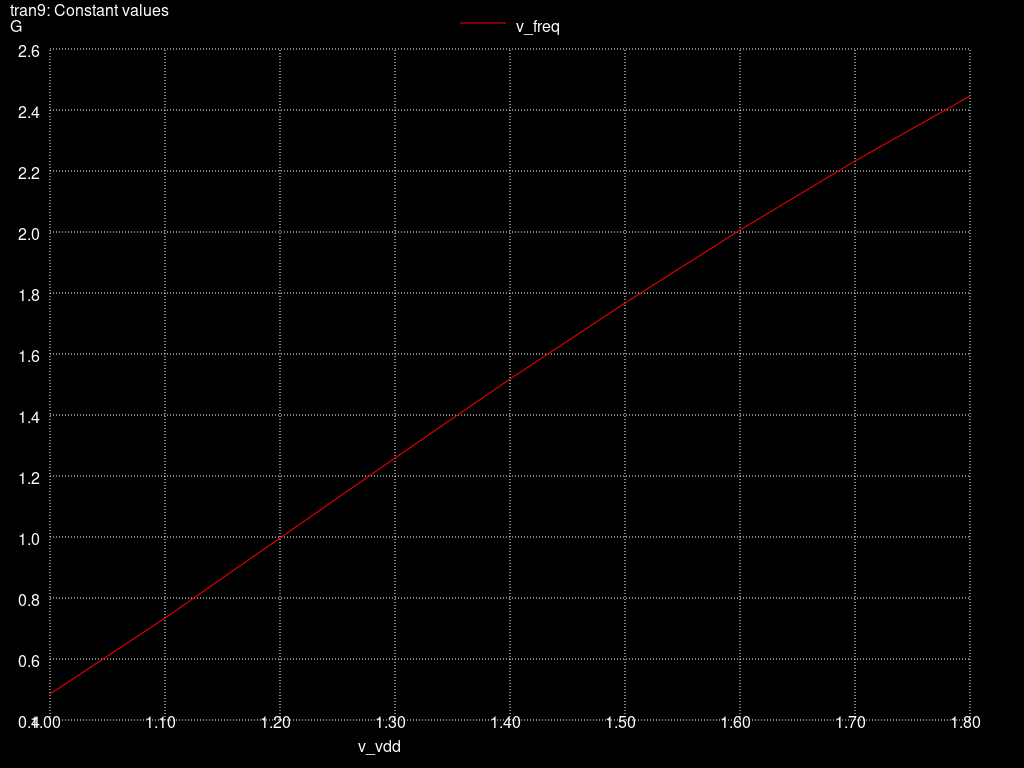
\includegraphics[width=0.47\linewidth]{tut5/reports/media/ro7.pre-layout.freq.png} &
     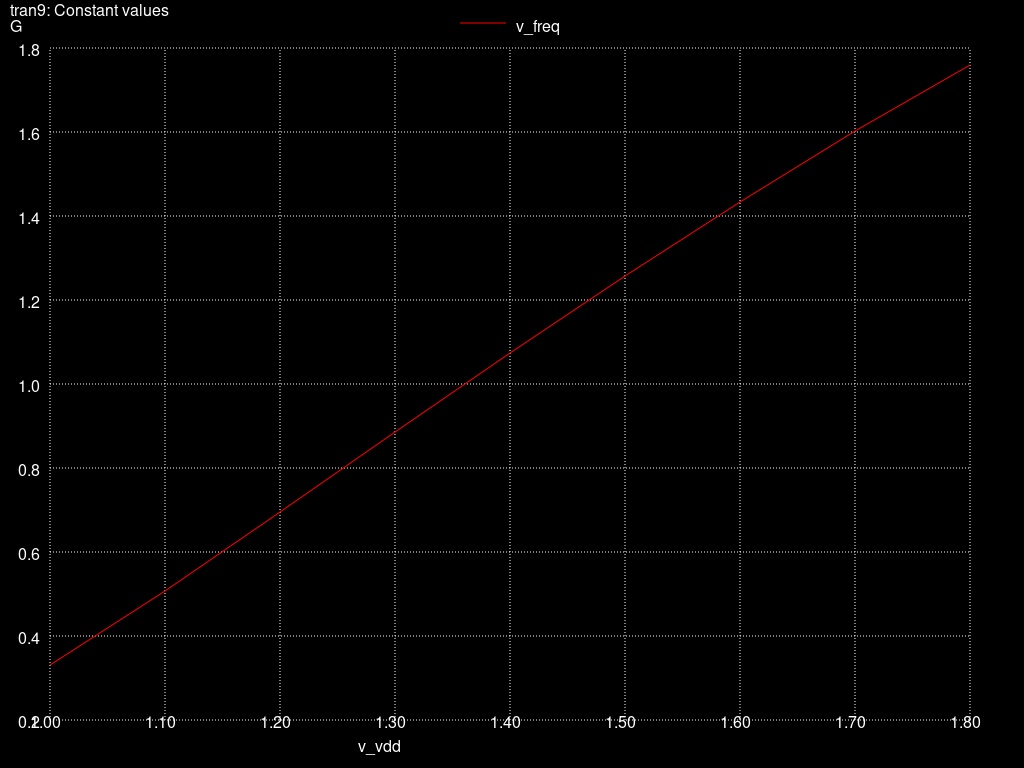
\includegraphics[width=0.47\linewidth]{tut5/reports/media/ro7.post-layout.freq.png} \\
     Fig 6a: Frequency of the circuit pre-layout & Fig 6b: Frequency of the circuit post-layout
\end{tabular}
\end{center}
\noindent We compare the obtained frequency and period values.
\begin{filecontents}{dly.dat}
X   $V_{DD}$    $prd-pre$   $prd-pos$   $freq-pre$  $freq-pos$
1	1	        2.06E-09	3.01E-09	4.85E+08	3.32E+08
2	1.1	      1.36E-09	1.97E-09	7.35E+08	5.08E+08
3	1.2	      1.00E-09	1.43E-09	1.00E+09	6.99E+08
4	1.3	      7.94E-10	1.12E-09	1.26E+09	8.93E+08
5	1.4	      6.59E-10	9.31E-10	1.52E+09	1.07E+09
6	1.5	      5.66E-10	7.95E-10	1.77E+09	1.26E+09
7	1.6	      4.98E-10	6.97E-10	2.01E+09	1.43E+09
8	1.7	      4.81E-10	6.24E-10	2.08E+09	1.60E+09
9	1.8	      4.09E-10	5.67E-10	2.44E+09	1.76E+09
\end{filecontents}

\begin{figure}[H]
\centering
\begin{tikzpicture}
\begin{axis}[
axis lines=middle,
ymin=0,
x label style={at={(current axis.right of origin)},anchor=north, below=10mm},
title={\textit{Frequency vs $V_{DD}$}},
    xlabel=$V_{DD}$ (V),
  ylabel=Frequency (s),
  % xticklabel style = {rotate=30,anchor=east},
  % xticklabel style = {anchor=below},
   enlargelimits = false,
  xticklabels from table={dly.dat}{$V_{DD}$},xtick=data]
\addplot[orange,thin,mark=square*] table [y=$freq-pre$,x=X]{dly.dat};
\addlegendentry{Period, pre-layout}
\addplot[blue,thin,mark=square*] table [y=$freq-pos$,x=X]{dly.dat};
\addlegendentry{Period, post-layout}]
% \addplot[red,thick,mark=square*] table [y=$freq-pre$,x=X]{dly.dat};
% \addlegendentry{$t_{p}$}]
\end{axis}
\end{tikzpicture} \\
Fig 7: A plot of the frequency of our seven-stage ring oscillator as a function of supply voltage.
\end{figure}
\begin{figure}[H]
\centering
\begin{tikzpicture}
\begin{axis}[
axis lines=middle,
ymin=0,
x label style={at={(current axis.right of origin)},anchor=north, below=10mm},
title={\textit{Period vs $V_{DD}$}},
    xlabel=$V_{DD}$ (V),
  ylabel=Delay (s),
  % xticklabel style = {rotate=30,anchor=east},
  % xticklabel style = {anchor=below},
   enlargelimits = false,
  xticklabels from table={dly.dat}{$V_{DD}$},xtick=data]
\addplot[orange,thin,mark=square*] table [y=$prd-pre$,x=X]{dly.dat};
\addlegendentry{Period, pre-layout}
\addplot[blue,thin,mark=square*] table [y=$prd-pos$,x=X]{dly.dat};
\addlegendentry{Period, post-layout}]
% \addplot[red,thick,mark=square*] table [y=$freq-pre$,x=X]{dly.dat};
% \addlegendentry{$t_{p}$}]
\end{axis}
\end{tikzpicture} \\
Fig 7: A plot of the period of our seven-stage ring oscillator as a function of supply voltage.
\end{figure}

\noindent We observe from the extracted spice netlists that the parasitics are distributed, but quite large around the \emph{DGND} pin. About an order of magnitude larger.

\section{Declarations}
\begin{enumerate}
    \item I have publicly hosted this work on GitHub to help reproduce all of my results. The same can be accessed through the following \href{https://github.com/iamkarthikbk/ee5311-2025}{\underline{link}}.
\end{enumerate}

\end{document}
